\begin{figure}[H]
    \centering
    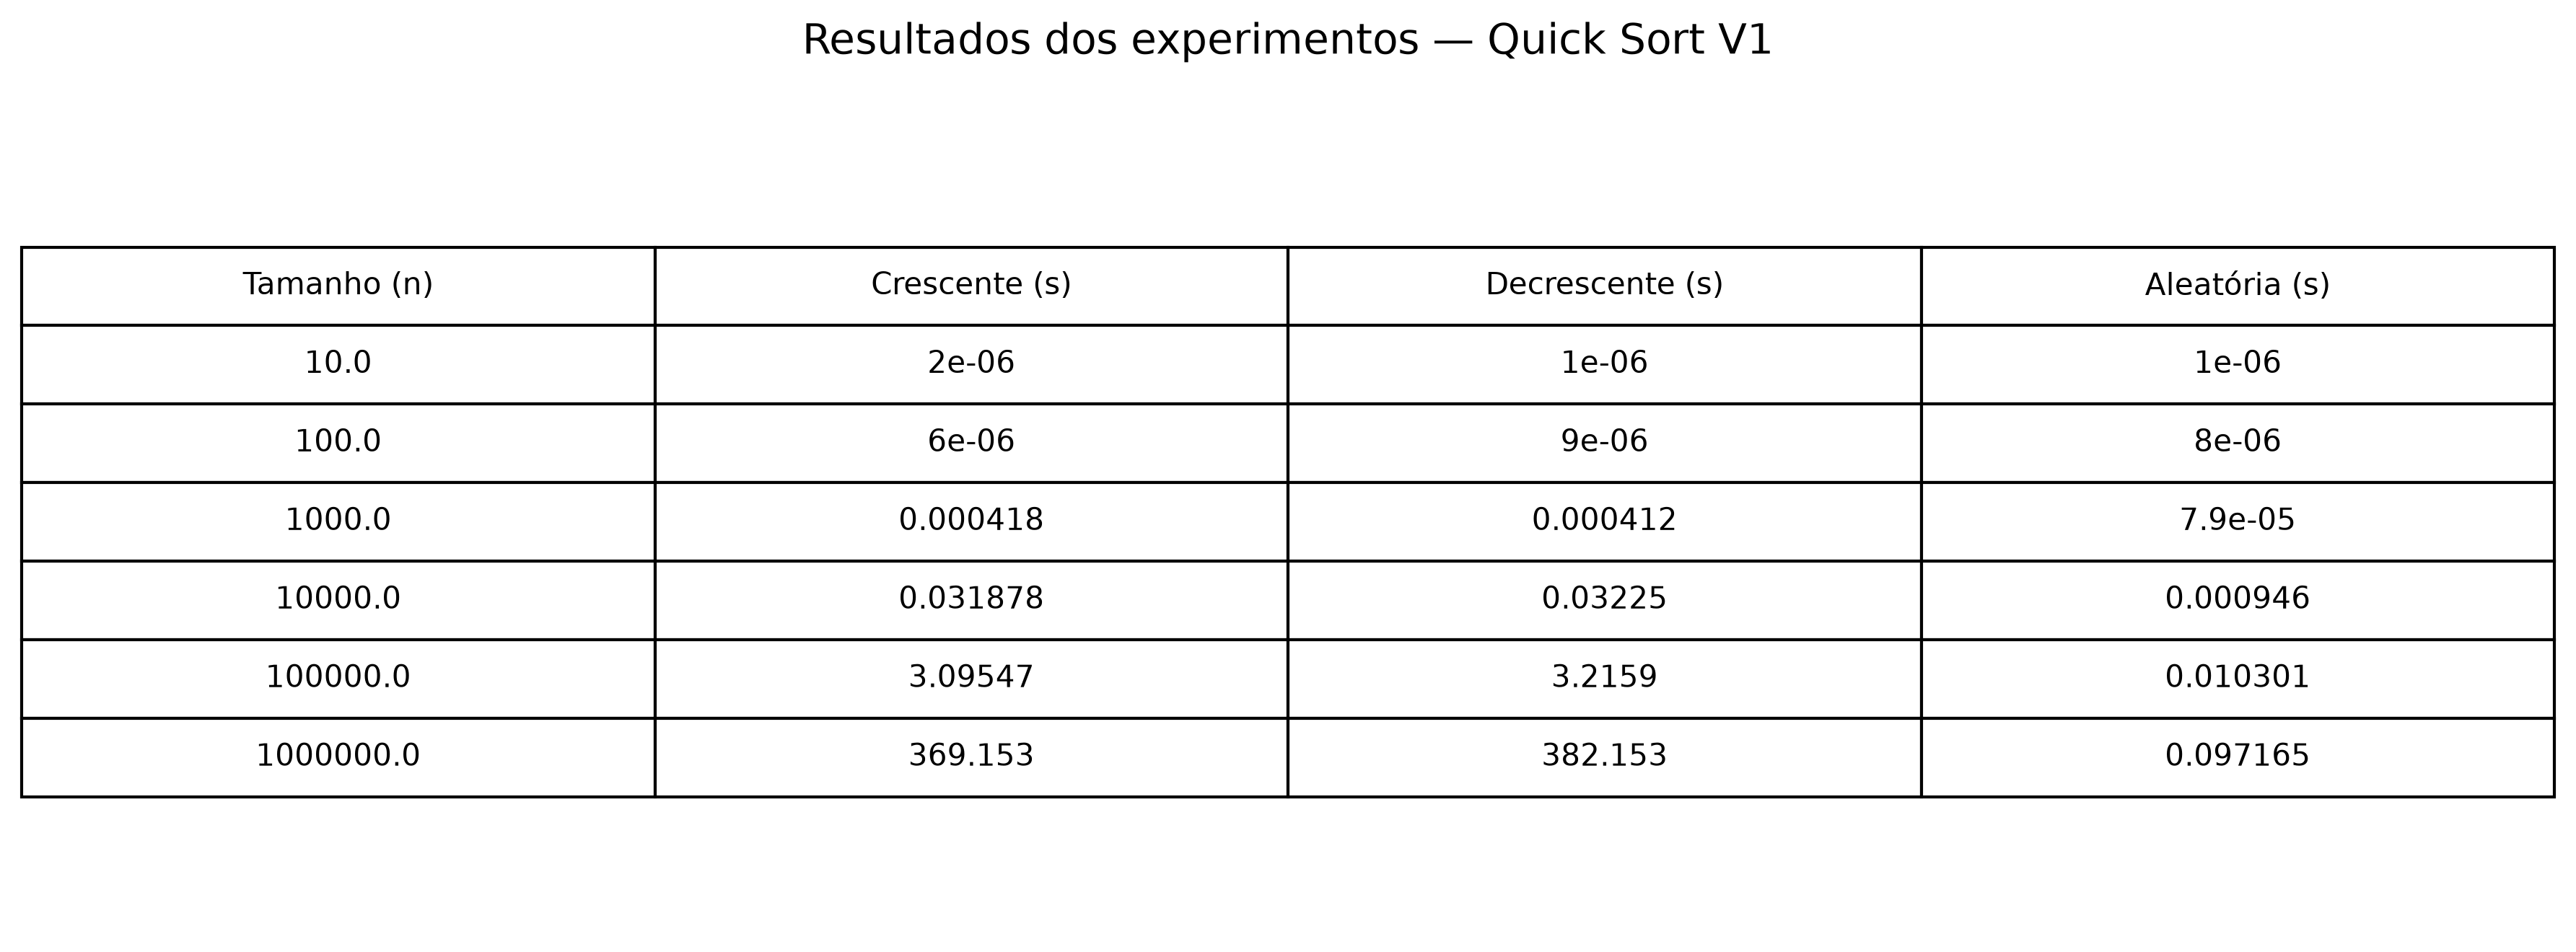
\includegraphics[width=16cm]{Imagens/Quick_Sort/tabela_v1.png}
    \caption{Tabela de tempo de execução do algoritmo Quick Sort (versão 1, pivô no primeiro elemento)}
    \label{fig:tabela-quick-v1}
\end{figure}

\begin{figure}[H]
    \centering
    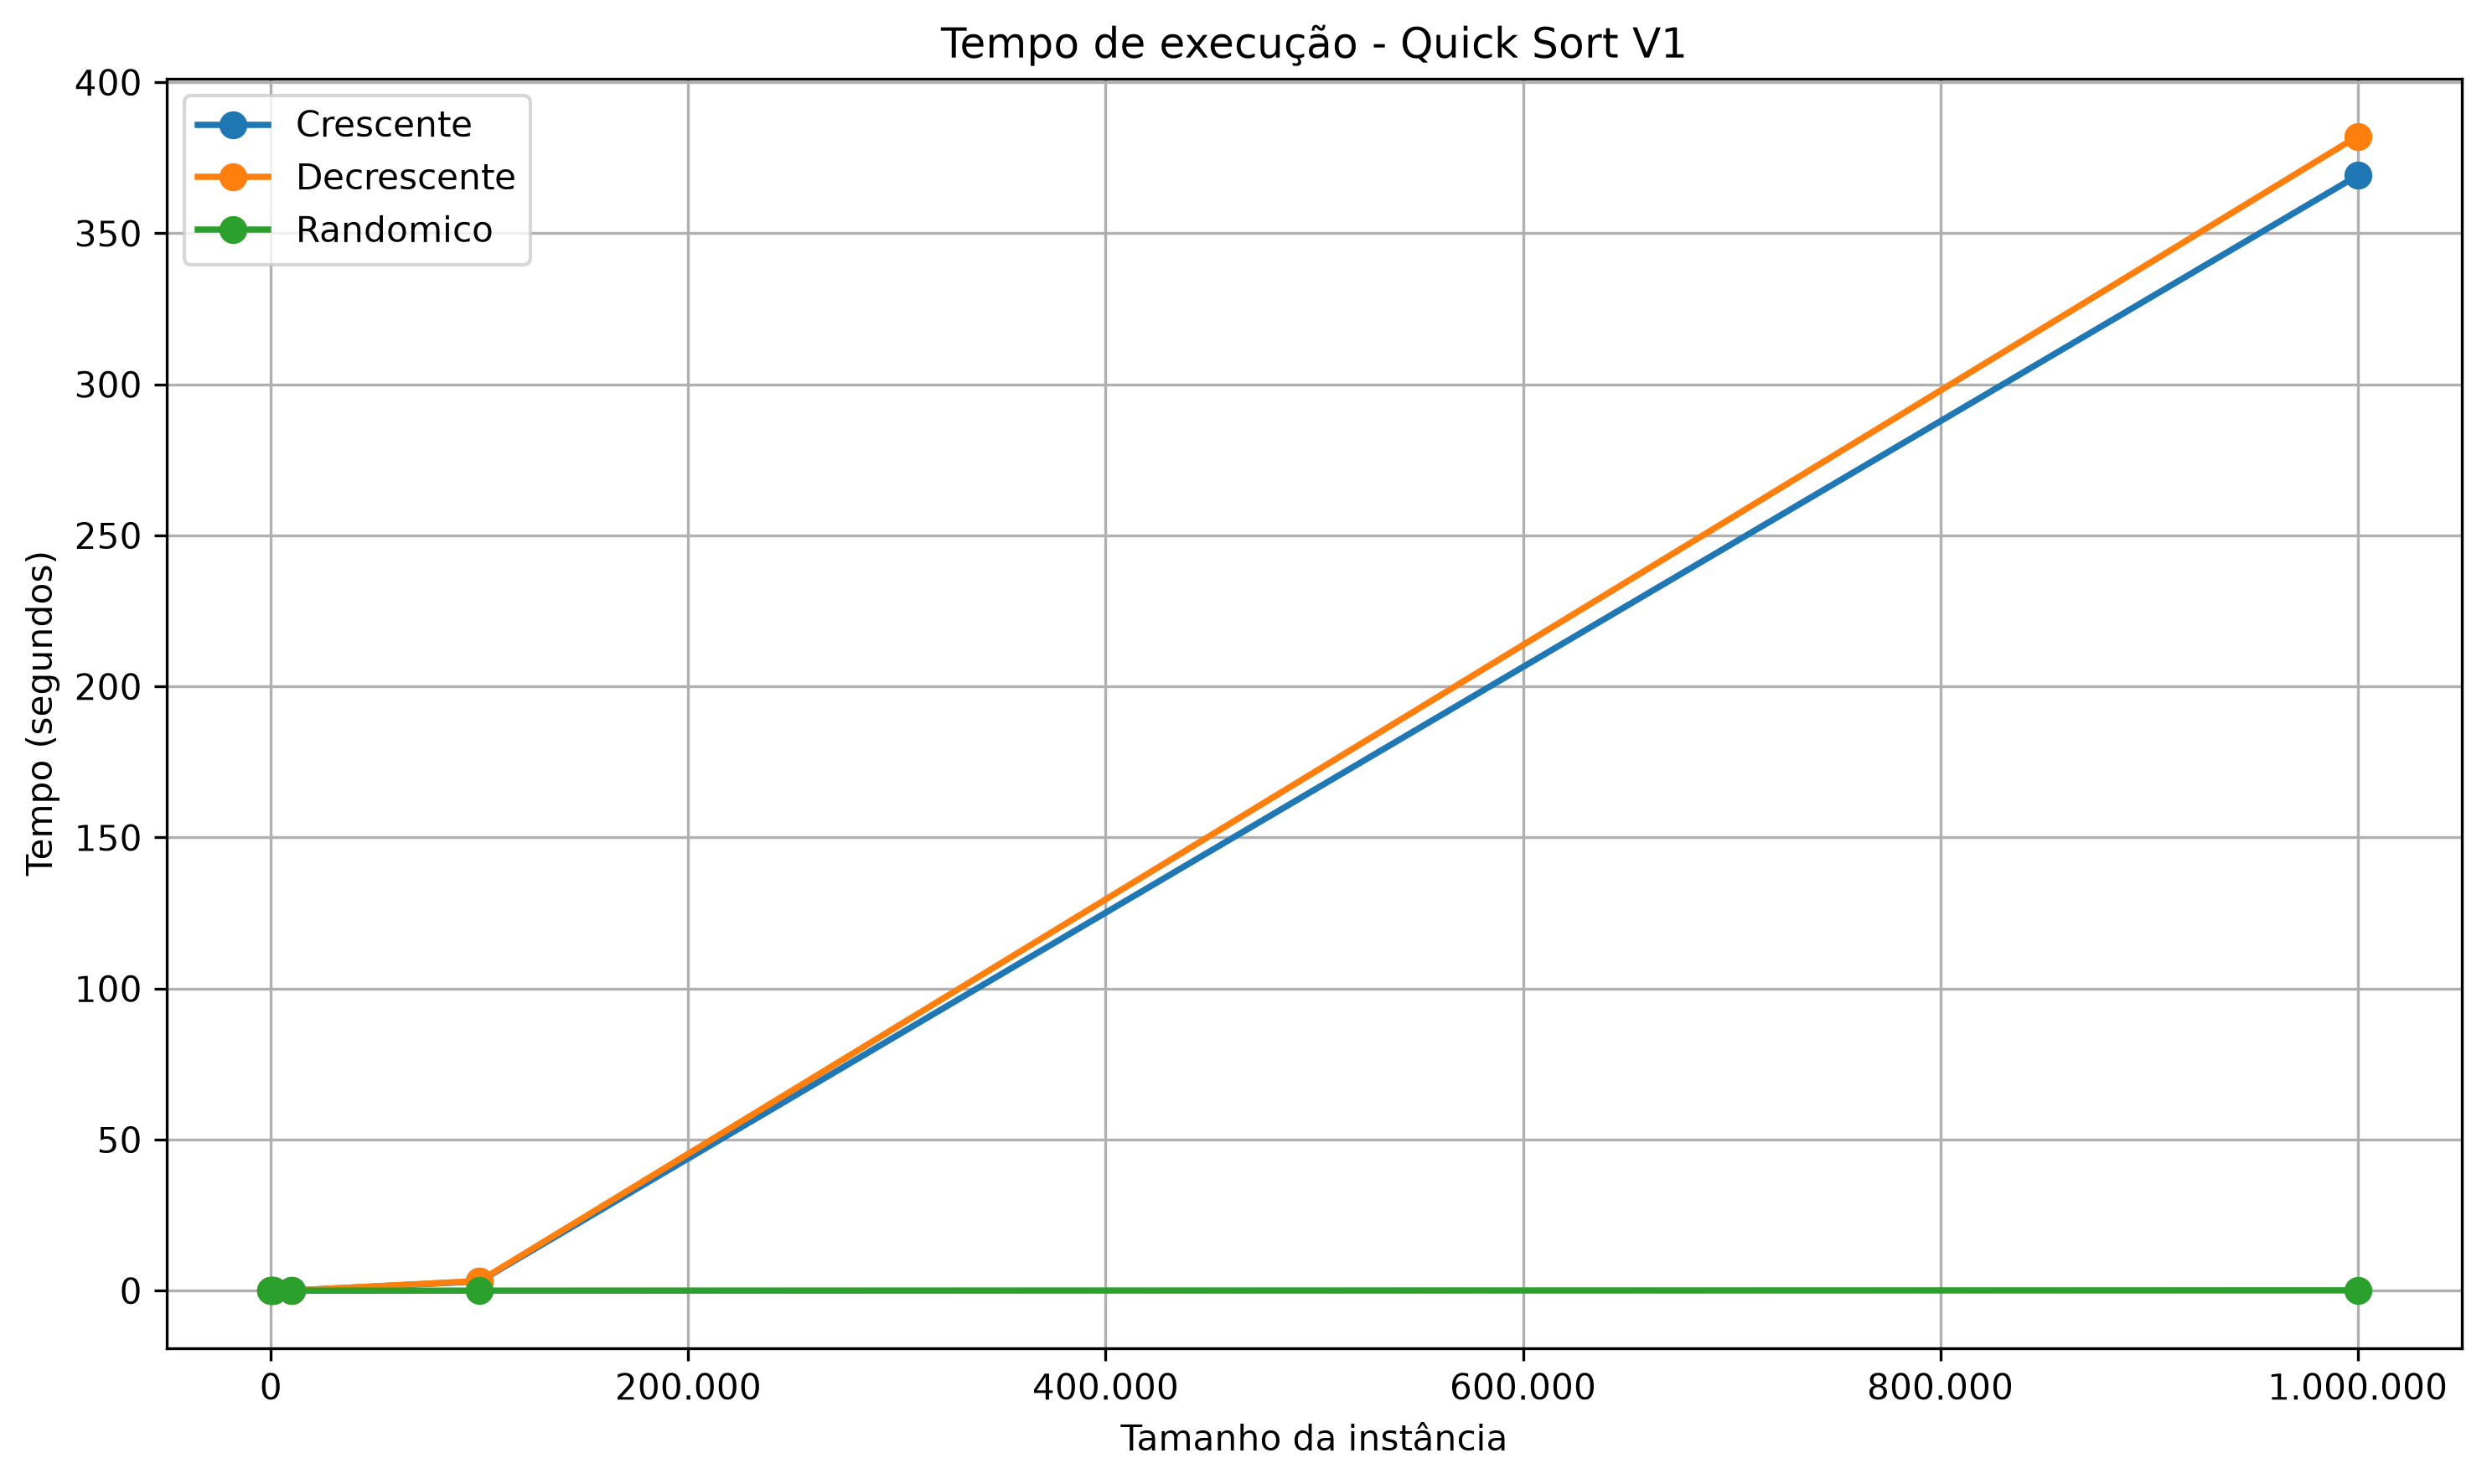
\includegraphics[width=10cm]{Imagens/Quick_Sort/grafico_v1.png}
    \caption{Gráfico de tempo de execução do algoritmo Quick Sort (versão 1, pivô no primeiro elemento)}
    \label{fig:grafico-quick-v1}
\end{figure}

\begin{figure}[H]
    \centering
    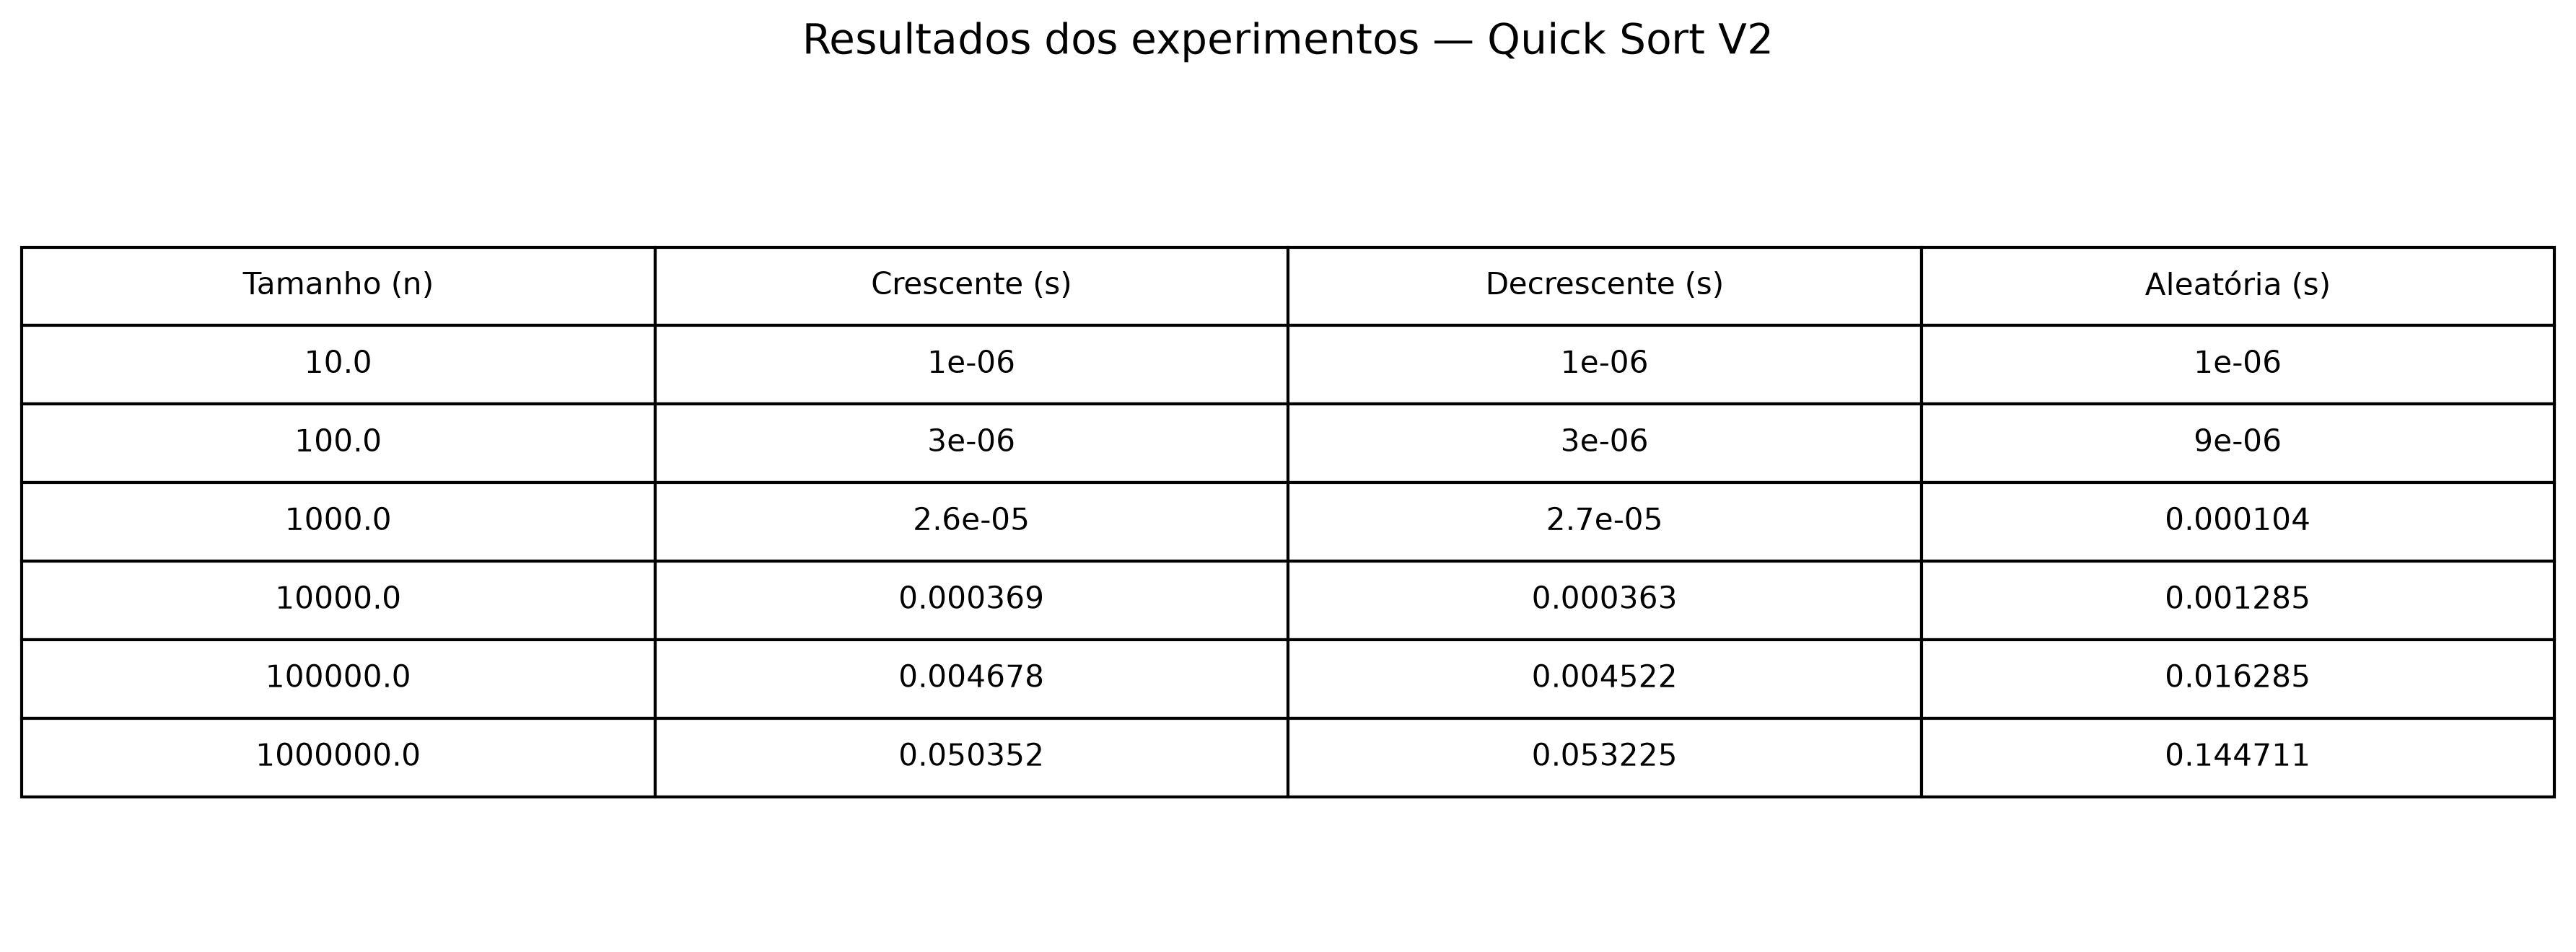
\includegraphics[width=16cm]{Imagens/Quick_Sort/tabela_v2.png}
    \caption{Tabela de tempo de execução do algoritmo Quick Sort (versão 2, pivô pela média aritmética)}
    \label{fig:tabela-quick-v2}
\end{figure}

\begin{figure}[H]
    \centering
    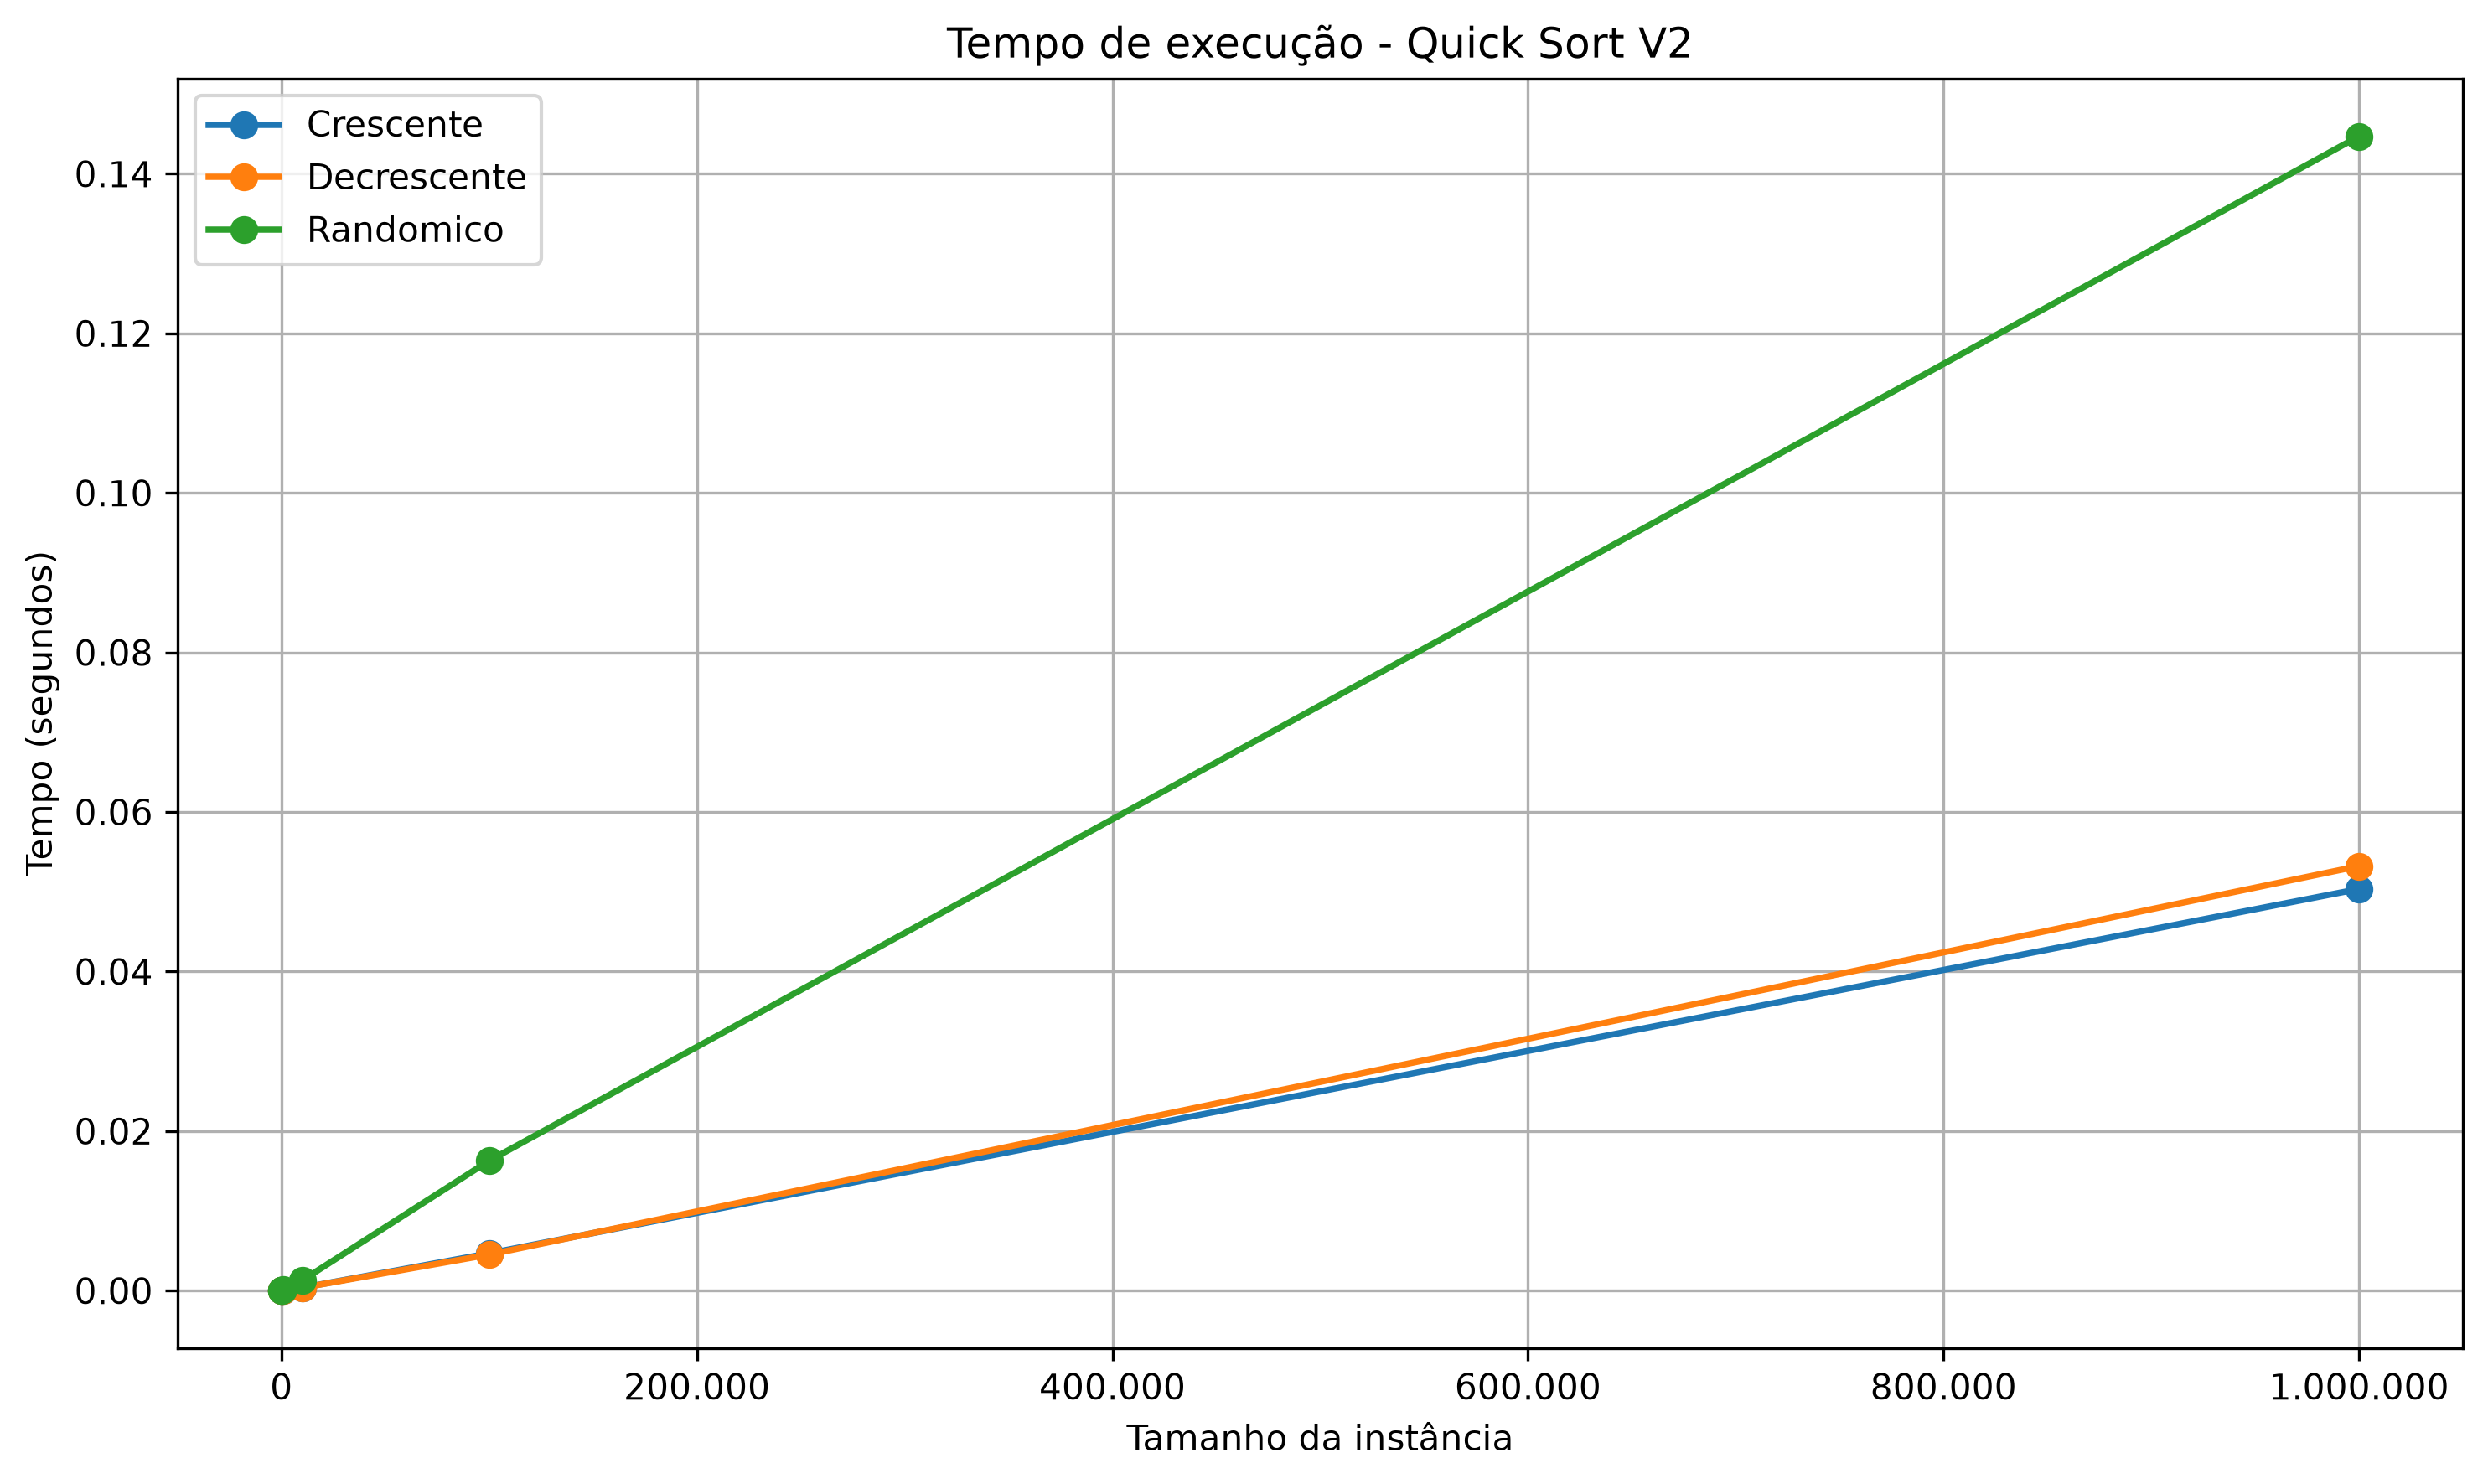
\includegraphics[width=10cm]{Imagens/Quick_Sort/grafico_v2.png}
    \caption{Gráfico de tempo de execução do algoritmo Quick Sort (versão 2, pivô pela média aritmética)}
    \label{fig:grafico-quick-v2}
\end{figure}

Os resultados obtidos nos experimentos estão apresentados nas tabelas e
nos gráficos de cada versão. Diferentemente do Merge Sort, o desempenho
do Quick Sort depende da organização inicial dos elementos, pois ela
influencia a escolha do pivô e, consequentemente, o balanceamento das
partições geradas a cada particionamento.

Na versão 1, o pivô é sempre o primeiro elemento da partição. Para
entradas aleatórias, é esperado que as partições fiquem razoavelmente
equilibradas, resultando em um comportamento próximo de
$\Theta(n\log n)$. Já para entradas crescentes e decrescentes, o pivô
tende a ser o menor ou o maior elemento da partição, gerando partições
muito desiguais e aproximando o algoritmo do pior caso, com complexidade
$\Theta(n^2)$. Esse efeito pode ser observado na
Figura~\ref{fig:grafico-quick-v1}, em que o tempo de execução dessas
entradas cresce de forma mais acentuada com o aumento do tamanho do
vetor.

Na versão 2, o pivô é a média aritmética dos elementos da partição. Como
a média tende a ficar próxima do centro dos valores quando eles estão
distribuídos de forma uniforme, as entradas crescentes e decrescentes
deixam de gerar partições tão desbalanceadas, e o tempo de execução
dessas entradas se aproxima do observado para entradas aleatórias, como
mostra a Figura~\ref{fig:grafico-quick-v2}. Em contrapartida, o cálculo
da média exige percorrer toda a partição a cada chamada, o que acrescenta
um custo linear adicional ao particionamento.

Comparando as duas versões, observa-se que a versão 2 reduz a
sensibilidade do algoritmo à ordem inicial do vetor, enquanto a versão 1
é mais simples e não possui custo adicional para a escolha do pivô, mas
é mais prejudicada por entradas já ordenadas. Para entradas aleatórias,
as duas versões apresentam comportamento semelhante, com a versão 2
ligeiramente mais custosa devido ao cálculo da média.

Além disso, o algoritmo realiza a ordenação no próprio vetor, sem
necessidade de vetores auxiliares. A implementação realiza a chamada
recursiva apenas sobre a menor partição, o que limita a profundidade da
pilha de recursão a, no máximo, proporcional a $\log_2 n$. Dessa forma,
o Quick Sort utiliza menos memória auxiliar do que o Merge Sort, embora
possa apresentar desempenho inferior em seu pior caso.